\documentclass[a4paper,14pt]{article}

% --- Настройка шрифтов и локализации для XeLaTeX ---
\usepackage{fontspec}
\usepackage{xunicode}
\usepackage{xltxtra}
\usepackage{polyglossia}
\setmainlanguage{russian}
\setotherlanguage{english}
\defaultfontfeatures{Ligatures=TeX}
\setmainfont{Times New Roman}
\newfontfamily\cyrillicfont{Times New Roman}
\setmonofont{Courier New}
\newfontfamily\cyrillicfonttt{Courier New}

% --- Математические пакеты ---
\usepackage{amsmath}
\usepackage{amssymb}

% --- Параметры страницы по ГОСТ (левое 3 см, правое 1 см, верхнее и нижнее по 2 см) ---
\usepackage[left=30mm, right=10mm, top=20mm, bottom=20mm]{geometry}

% --- Интервалы и абзацный отступ (1.25 см, 1.5 интервал) ---
\usepackage{indentfirst}
\setlength{\parindent}{1.25cm}
\usepackage{setspace}
\onehalfspacing

% --- Пакеты для таблиц, списков и графики ---
\usepackage{tabularx}
\usepackage{booktabs}
\usepackage{array}
\usepackage{enumitem}
\setlist{nosep, leftmargin=\parindent}
\usepackage{graphicx}
\usepackage{tikz}
\usetikzlibrary{shapes.geometric, arrows, positioning}

% --- Листинги кода с корректным отображением кириллицы и пробелов ---
\usepackage{listings}
\usepackage{xcolor}

\lstset{
    basicstyle=\ttfamily\footnotesize,
    columns=flexible,
    keepspaces=true,
    breaklines=true,
    frame=single,
    tabsize=2,
    showstringspaces=false,
    keywordstyle=\bfseries\color{blue!70!black},
    commentstyle=\itshape\color{green!50!black},
    stringstyle=\color{red!60!black},
    numbers=none
}

\lstdefinelanguage{bash}{
  keywords={sudo, systemctl, pg_basebackup, pg_dump, pg_restore, psql, crontab, cp, rm, mv, mkdir, chown, chmod, pg_waldump, touch, cat},
  morecomment=[l]{\#},
  morestring=[b]',
  morestring=[b]"
}

% --- Оформление заголовков по стандарту ---
\usepackage{titlesec}
\titleformat{\section}[block]
  {\normalfont\bfseries\filright}
  {\hspace{1.25cm}\thesection\quad}
  {0pt}
  {\MakeUppercase}

\titleformat{\subsection}[block]
  {\normalfont\bfseries\filright}
  {\hspace{1.25cm}\thesubsection\quad}
  {0pt}
  {}

\titlespacing*{\section}{0pt}{18pt}{12pt}
\titlespacing*{\subsection}{0pt}{12pt}{6pt}

% Настройка подписей к рисункам и таблицам
\usepackage[tableposition=top,figureposition=bottom]{caption}
\DeclareCaptionLabelSeparator{emdash}{~---~}
\captionsetup[figure]{
  name={Рисунок},
  labelsep=emdash,
  font={small},
  justification=centering,
  singlelinecheck=true
}
\captionsetup[table]{
  name={Таблица},
  labelsep=emdash,
  font={small},
  justification=raggedright,
  singlelinecheck=false
}

% --- Отточие в содержании ---
\usepackage{tocloft}
\renewcommand{\cftsecleader}{\cftdotfill{\cftdotsep}}
\renewcommand{\cfttoctitlefont}{\hfill\bfseries\MakeUppercase}
\renewcommand{\cftaftertoctitle}{\hfill}

\begin{document}

% =========================================================================
% ТИТУЛЬНЫЙ ЛИСТ
% =========================================================================
\begin{titlepage}
    \centering
    {\small МИНИСТЕРСТВО НАУКИ И ВЫСШЕГО ОБРАЗОВАНИЯ РОССИЙСКОЙ ФЕДЕРАЦИИ}\\
    {\scriptsize \textbf{ФЕДЕРАЛЬНОЕ ГОСУДАРСТВЕННОЕ АВТОНОМНОЕ ОБРАЗОВАТЕЛЬНОЕ УЧРЕЖДЕНИЕ ВЫСШЕГО ОБРАЗОВАНИЯ}}\\
    {\bfseries «НАЦИОНАЛЬНЫЙ ИССЛЕДОВАТЕЛЬСКИЙ УНИВЕРСИТЕТ ИТМО»}\\[0.8cm]

    \textbf{Факультет безопасности информационных технологий}\\[0.6cm]

    \textbf{Направление подготовки: 10.03.01 Информационная безопасность} \\
    \textbf{Образовательная программа: «Технологии защиты информации»} \\[0.6cm]

    \textbf{Дисциплина:} \\
    \textit{\textbf{«Информационная безопасность баз данных»}} \\ [1.5cm]

    {\bfseries ОТЧЕТ ПО ЛАБОРАТОРНОЙ РАБОТЕ №5}\\
    \textit{{\bfseries «Резервирование БД и восстановление по контрольным точкам»}}\\[3.5cm]

    \begin{flushright}
        \textbf{Выполнил студент(ы):} \\ [0.5em]
        группа.поток ИББД 1.7 \\ [0.5em]
        Пахомов Владимир Юрьевич / \raisebox{-0.3\height}{
\includegraphics[width=1.3cm]{sign1.png}} \\
        {\scriptsize{\textit{ФИО \hspace{2cm} Подпись \hspace{0.3cm}}}} \\ [0.3cm]
        Сивков Иван Александрович / \raisebox{-0.4\height}{
\includegraphics[width=1.1cm]{sign2.jpg}} \\
        {\scriptsize{\textit{ФИО \hspace{2cm} Подпись \hspace{0.3cm}}}} \\ [0.3cm]
        Булин Михаил Михайлович / \raisebox{-0.4\height}{
\includegraphics[width=1.3cm]{sign3.png}} \\
        {\scriptsize{\textit{ФИО \hspace{2cm} Подпись \hspace{0.3cm}}}} \\ [0.3cm]


        \textbf{Проверил:}\\ [0.5em]
        Ярцева Наталия Андреевна / \underline{\hspace{1.5cm}} \\
        {\scriptsize{\textit{ФИО \hspace{2cm} Подпись \hspace{1cm}}}} \\ [1.5cm]

        {\scriptsize \underline{\hspace{4cm}}} \\
        {\scriptsize \textit{Отметка о выполнении (один из вариантов: \\ отлично, хорошо, удовлетворительно, зачтено)}} \\
        {\scriptsize \underline{\hspace{4cm}}} \\
        {\scriptsize \textit{Дата \hspace{1.5cm}}}
    \end{flushright}

    \vfill
    Санкт-Петербург\\
    2026
\end{titlepage}

% =========================================================================
% СОДЕРЖАНИЕ
% =========================================================================
\newpage
\pagestyle{plain}
\setcounter{page}{2}

\begin{center}
    {\bfseries \MakeUppercase{Содержание}}
\end{center}
\vspace{-0.5cm}
\tableofcontents

% =========================================================================
% ВВЕДЕНИЕ
% =========================================================================
\newpage
\begin{center}
    {\bfseries \MakeUppercase{Введение}}
\end{center}
\addcontentsline{toc}{section}{ВВЕДЕНИЕ}

\textbf{Цель работы}: получение практических навыков разработки политик и регламентов резервного копирования баз данных, настройки механизмов непрерывной архивации журналов упреждающей записи (Write-Ahead Logging, WAL), моделирования инцидентов деструктивной модификации данных, проведения аварийного восстановления на определенный момент времени (Point-In-Time Recovery, PITR) до контрольной точки, а также последующего криминалистического анализа аннулированных изменений.

Обеспечение доступности и целостности информации выступает ключевой задачей информационной безопасности в соответствии с базовой триадой CIA (Confidentiality, Integrity, Availability). В автоматизированной информационной системе морских контейнерных перевозок непреднамеренные программные сбои или несанкционированные воздействия на таблицы рейсов, заказов и контейнеров способны парализовать логистические процессы морского терминала.

В рамках лабораторной работы на базе созданной в ЛР1--4 СУБД PostgreSQL (\texttt{container\_cargo\_db}) решаются четыре основные задачи:
\begin{enumerate}
    \item организация регулярного создания резервных копий по расписанию с непрерывной архивацией журналов WAL;
    \item установка именованной контрольной точки восстановления (\textit{Restore Point}) и внесение случайных деструктивных изменений в таблицы БД;
    \item проведение процедуры отката состояния СУБД к созданной контрольной точке (PITR);
    \item анализ возможности просмотра и аудита откаченных изменений с помощью системы логирования СУБД (\texttt{main\_log} из ЛР3) и средств системы резервирования (\texttt{pg\_waldump}).
\end{enumerate}

% =========================================================================
% 1. РЕЗЕРВНОЕ КОПИРОВАНИЕ БД ПО РАСПИСАНИЮ
% =========================================================================
\newpage
\section{Создание резервной копии БД согласно расписанию}

В соответствии с заданием организуем регулярное резервное копирование базы данных по расписанию с использованием утилиты \texttt{pg\_basebackup} и механизмов непрерывной архивации журналов предзаписи (Write-Ahead Logging, WAL).

Для включения архивации транзакционных журналов в конфигурацию СУБД внесены следующие параметры:

\begin{lstlisting}[language=SQL]
ALTER SYSTEM SET wal_level = 'replica';
ALTER SYSTEM SET archive_mode = 'on';
ALTER SYSTEM SET archive_command = 'test ! -f /var/backups/postgres/wal_archive/%f && cp %p /var/backups/postgres/wal_archive/%f';
ALTER SYSTEM SET archive_timeout = 900;
\end{lstlisting}

Автоматическое создание физических снимков настроено с помощью системного планировщика \texttt{cron} для пользователя \texttt{postgres} (запуск ежедневно в 02:00 ночи):

\begin{lstlisting}[language=bash]
# Расписание в crontab
0 2 * * * pg_basebackup -h localhost -U postgres -D /var/backups/postgres/base_backups/base_backup -Ft -z -X fetch
\end{lstlisting}

Подтверждение настройки расписания в планировщике и параметров архивации приведено на рисунке \ref{fig:screen1}.

\begin{figure}[h!]
    \centering
    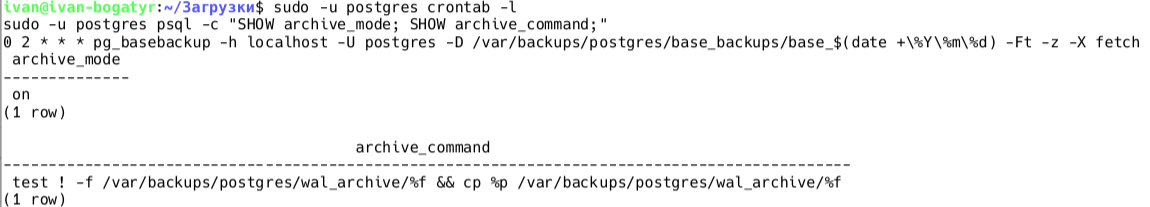
\includegraphics[width=0.9\textwidth]{screen1_cron.png}
    \caption{Настройка планировщика cron и параметров архивации WAL}
    \label{fig:screen1}
\end{figure}

% =========================================================================
% 2. ФИКСАЦИЯ КОНТРОЛЬНОЙ ТОЧКИ И ВНЕСЕНИЕ ИЗМЕНЕНИЙ
% =========================================================================
\newpage
\section{Фиксация контрольной точки и внесение изменений}

\subsection{Создание базового снимка и контрольной точки}
Перед проведением эксперимента сформирован актуальный базовый физический снимок каталога данных:
\begin{lstlisting}[language=bash]
sudo -u postgres pg_basebackup -h localhost -D /var/backups/postgres/base_backups/base_snapshot -Fp -Xs -P
\end{lstlisting}

Затем администратор СУБД фиксирует эталонное состояние данных и создает именованную контрольную точку восстановления (\textit{Restore Point}):
\begin{lstlisting}[language=SQL]
SELECT id, cargo_name, total_price, cargo_weight FROM orders LIMIT 3;
SELECT pg_create_restore_point('rp_cargo_safe_state');
\end{lstlisting}

Результат фиксации исходных цен и создания контрольной точки представлен на рисунке \ref{fig:screen2}.

\begin{figure}[h!]
    \centering
    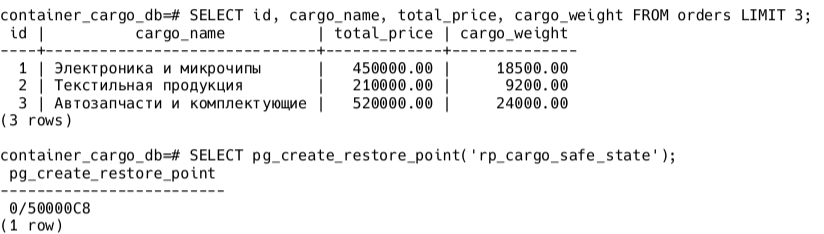
\includegraphics[width=0.9\textwidth]{screen2_restore_point.png}
    \caption{Фиксация исходных цен и создание контрольной точки rp\_cargo\_safe\_state}
    \label{fig:screen2}
\end{figure}

\subsection{Внесение деструктивных изменений}
Смоделируем компрометацию учетной записи: обнуление цен заказов, удаление контейнеров и внедрение фиктивного контрагента:

\begin{lstlisting}[language=SQL]
UPDATE orders SET total_price = 0.00, cargo_weight = 1.00 WHERE id IN (1, 2, 3);
DELETE FROM order_containers WHERE id IN (1, 2, 3);
INSERT INTO clients (name, email, phone, address)
VALUES ('Phantom Logistics Ltd.', 'hacker@darknet.io', '+000-000-0000', 'Unknown Island 99');
SELECT pg_switch_wal();
\end{lstlisting}

Фиксация поврежденных данных (обнуленные цены и искаженный вес) и автоматическое срабатывание триггера аудита \texttt{main\_log} (разработанного в ЛР3) показаны на рисунке \ref{fig:screen3}.

\begin{figure}[h!]
    \centering
    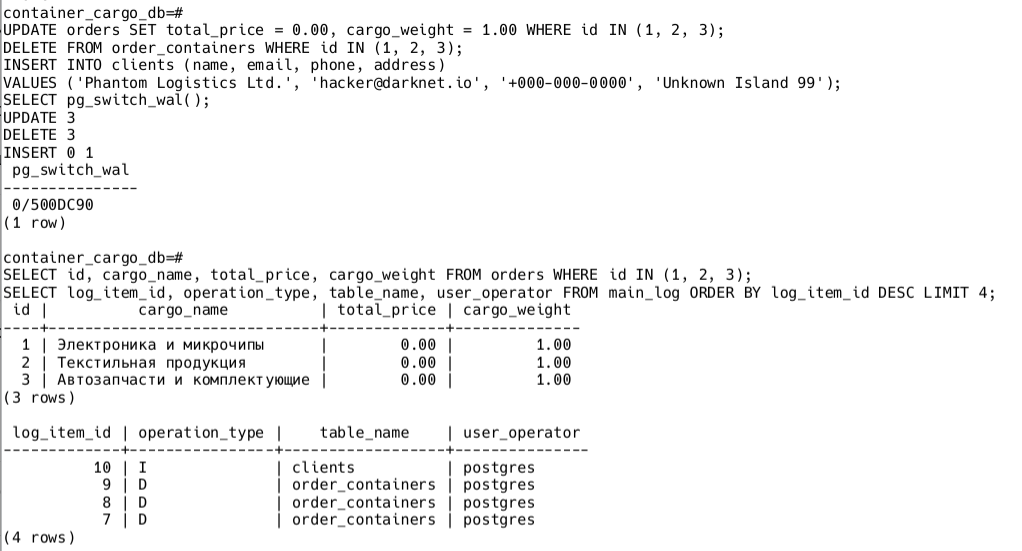
\includegraphics[width=0.95\textwidth]{screen3_corrupted.png}
    \caption{Отражение повреждения данных (цены 0.00) и аудит операций в main\_log}
    \label{fig:screen3}
\end{figure}

% =========================================================================
% 3. ОТКАТ К КОНТРОЛЬНОЙ ТОЧКЕ (PITR)
% =========================================================================
\newpage
\section{Откат к контрольной точке (Point-In-Time Recovery)}

\subsection{Процедура восстановления}
Откат состояния СУБД производится через процедуру аварийного восстановления на определенный момент времени:

\begin{lstlisting}[language=bash]
sudo systemctl stop postgresql
sudo mv /var/lib/postgresql/16/main /var/lib/postgresql/16/main_corrupted
sudo cp -r /var/backups/postgres/base_backups/base_snapshot /var/lib/postgresql/16/main
sudo chown -R postgres:postgres /var/lib/postgresql/16/main

sudo -u postgres touch /var/lib/postgresql/16/main/recovery.signal
sudo -u postgres bash -c 'cat >> /var/lib/postgresql/16/main/postgresql.auto.conf' << 'EOF'
restore_command = 'cp /var/backups/postgres/wal_archive/%f %p'
recovery_target_name = 'rp_cargo_safe_state'
recovery_target_action = 'promote'
EOF

sudo systemctl start postgresql
\end{lstlisting}

\subsection{Проверка целостности восстановленных данных}
После запуска СУБД накатывает сегменты WAL из архива ровно до созданной контрольной точки. Выполним проверку состояния таблиц:

\begin{lstlisting}[language=SQL]
SELECT id, cargo_name, total_price, cargo_weight FROM orders WHERE id IN (1, 2, 3);
SELECT id, order_id, container_id, seal_number FROM order_containers WHERE id IN (1, 2, 3);
SELECT * FROM clients WHERE email = 'hacker@darknet.io';
\end{lstlisting}

Результат проверки представлен на рисунке \ref{fig:screen4}. Все цены и контейнеры вернулись в исходное состояние, фиктивный контрагент удален.

\begin{figure}[h!]
    \centering
    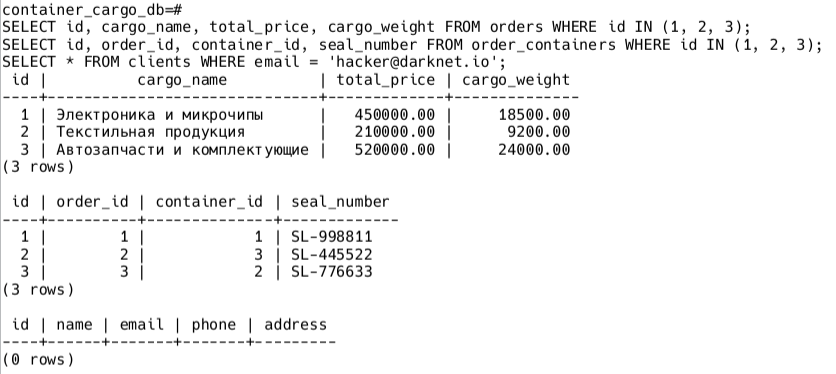
\includegraphics[width=0.95\textwidth]{screen4_restored.png}
    \caption{Успешное восстановление данных к контрольной точке rp\_cargo\_safe\_state}
    \label{fig:screen4}
\end{figure}

% =========================================================================
% 4. АНАЛИЗ И АУДИТ ОТКАЧЕННЫХ ИЗМЕНЕНИЙ
% =========================================================================
\newpage
\section{Анализ откаченных изменений}

\subsection{Анализ с помощью системы логирования СУБД (ЛР3)}
При откате базы данных таблица \texttt{public.main\_log} также откатывается в состояние до инцидента. Следовательно, при классическом PITR внутренний журнал аудита не содержит записей о совершенных деструктивных действиях. Для расследования инцидентов журнал должен выгружаться из сохраненной копии \texttt{main\_corrupted} до ее перезаписи.

\subsection{Анализ с помощью средств системы резервирования (pg\_waldump)}
Файлы архивных журналов в директории \texttt{wal\_archive} сохраняются независимо от процедур отката базы. С помощью утилиты \texttt{pg\_waldump} выполнено декодирование архивного WAL-файла, содержащего события после контрольной точки:

\begin{lstlisting}[language=bash]
sudo pg_waldump /var/backups/postgres/wal_archive/000000010000000000000005 | grep -E "RESTORE_POINT|Heap"
\end{lstlisting}

Вывод утилиты приведен на рисунке \ref{fig:screen5}.

\begin{figure}[h!]
    \centering
    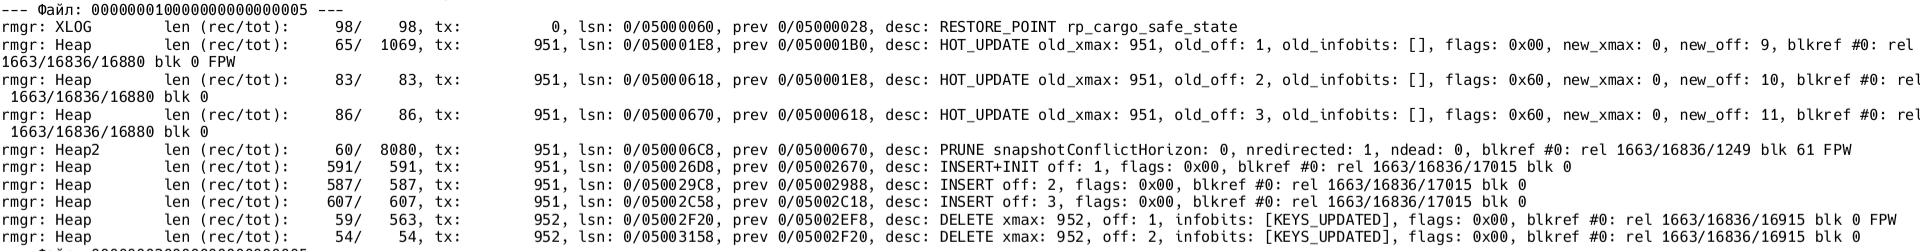
\includegraphics[width=1.0\textwidth]{screen5_waldump.png}
    \caption{Декодирование журнала WAL утилитой pg\_waldump (контрольная точка и откаченные операции)}
    \label{fig:screen5}
\end{figure}

В журнале четко идентифицируются:
\begin{itemize}
    \item маркер контрольной точки \texttt{RESTORE\_POINT rp\_cargo\_safe\_state};
    \item транзакции \texttt{HOT\_UPDATE} по обнулению стоимостей заказов;
    \item операции \texttt{INSERT} и \texttt{DELETE} по удалению связей контейнеров.
\end{itemize}

% =========================================================================
% ЗАКЛЮЧЕНИЕ
% =========================================================================
\newpage
\begin{center}
    {\bfseries \MakeUppercase{Заключение}}
\end{center}
\addcontentsline{toc}{section}{ЗАКЛЮЧЕНИЕ}

В ходе выполнения лабораторной работы были освоены и практически применены технологии резервирования, обеспечения высокой доступности и аварийного восстановления реляционной базы данных «Информационная система морских контейнерных перевозок» в СУБД PostgreSQL.

В рамках работы достигнуты следующие результаты:
\begin{enumerate}
    \item Разработан регламент резервного копирования данных, включающий создание физических снимков (\texttt{pg\_basebackup}) и непрерывную архивацию журналов предзаписи (\texttt{WAL-archiving}); процесс автоматизирован посредством планировщика \texttt{cron}.
    \item Введена в эксплуатацию именованная контрольная точка восстановления \texttt{rp\_cargo\_safe\_state}, зафиксировавшая эталонное состояние таблиц базы данных.
    \item Смоделирован сценарий деструктивного нарушения целостности данных (обнуление цен, удаление связей контейнеров, внедрение фиктивных записей контрагентов).
    \item Успешно выполнен процесс отката базы данных к контрольной точке по технологии Point-In-Time Recovery (PITR); верифицировано восстановление целостности данных.
    \item Проведен комплексный анализ аннулированных транзакций: раскрыта специфика поведения встроенной таблицы-лога (\texttt{main\_log}) при откате кластера и продемонстрирован независимый метод форензик-анализа через декодирование архивных сегментов WAL утилитой \texttt{pg\_waldump}.
\end{enumerate}

\end{document}
